% AI Assistance Disclosure: Claude Code (Opus 5.5), 2026-10-19.
% Scope: Four-page learning-support guide to the existing Pub/Sub interactions and
% containerization of the repository. Condensed from guide-detailed.tex (kept in this
% folder). Documentation only; no implementation or design decisions. Author review: Pending.
\documentclass[11pt,a4paper]{article}
\PassOptionsToPackage{hyphens,obeyspaces,spaces}{url}
\usepackage[a4paper,margin=1.7cm,top=1.5cm,bottom=1.6cm]{geometry}
\usepackage[T1]{fontenc}
\usepackage{lmodern}
\usepackage{microtype}
\usepackage{xcolor}
\usepackage{tikz}
\usetikzlibrary{arrows.meta,positioning,calc}
\usepackage{enumitem}
\usepackage{booktabs}
\usepackage{titlesec}
\usepackage[hidelinks]{hyperref}

\definecolor{accent}{HTML}{1F5FAD}
\definecolor{sync}{HTML}{2E7D32}
\definecolor{async}{HTML}{C2410C}
\definecolor{topic}{HTML}{FDE7D6}
\definecolor{svc}{HTML}{E3EDF9}
\definecolor{infra}{HTML}{F1F1F1}
\definecolor{note}{HTML}{FFF8E1}

\setlength{\parindent}{0pt}
\setlength{\parskip}{4pt plus 1pt}
\setlength{\emergencystretch}{3em}
\setlist{itemsep=1pt,topsep=2pt,parsep=0pt,leftmargin=1.2em}
\titleformat{\section}{\large\bfseries\color{accent}}{\thesection}{0.5em}{}
\titlespacing*{\section}{0pt}{8pt}{3pt}
\pagestyle{plain}
\setlength{\textfloatsep}{8pt plus 2pt}
\setlength{\floatsep}{6pt}
\setlength{\abovecaptionskip}{3pt}
\setlength{\belowcaptionskip}{0pt}
\renewcommand{\footnotesize}{\fontsize{8.5}{10}\selectfont}

\urlstyle{tt}
\makeatletter
\g@addto@macro\UrlBreaks{\do\-\do\_\do\.\do\:\do\=}
\makeatother
\Urlmuskip=0mu
\newcommand{\code}[1]{\nolinkurl{#1}}

\tikzset{
  >={Stealth[length=2.2mm]},
  svcbox/.style={draw=accent!70!black, fill=svc, rounded corners=2pt, align=center,
    font=\small, inner sep=2pt},
  topicbox/.style={draw=async!80!black, fill=topic, rounded corners=5pt, align=center,
    font=\small\ttfamily, inner sep=2pt},
  subbox/.style={draw=black!45, fill=infra, rounded corners=1pt, align=left,
    font=\footnotesize, inner sep=2pt, anchor=west},
  asynca/.style={->, draw=async, thick},
  synca/.style={->, draw=sync, thick},
  lbl/.style={font=\small, fill=white, inner sep=1pt},
  life/.style={draw=black!30, dashed},
  head/.style={draw=black!60, fill=svc, rounded corners=2pt, align=center,
    font=\small\bfseries, minimum width=25mm, minimum height=8mm, inner sep=1pt},
  m/.style={->, thick, draw=async},
  mh/.style={->, thick, draw=sync},
  mlab/.style={font=\small, above, inner sep=1pt},
  act/.style={font=\small, align=left, fill=note, draw=black!25, inner sep=1.5pt},
}

\hypersetup{pdftitle={FoC services: Pub/Sub interactions and containers (short guide)}}

\begin{document}

{\raggedright\Large\bfseries\color{accent} How the seven FoC services talk over Pub/Sub, and how each is containerized\par}
\vspace{2pt}
{\small A four-page teaching guide to the CS3219 P32 repository, 19 October 2026.\footnote{Grounded
in the code at \code{ea16eec} (\code{main}); the service code is unchanged at \code{7e8c31b}, which adds
only the event bus tap and these docs. File and line evidence for every claim is in
\code{CLAIM_MAP.md}; the full 33-page version, with payload examples and Cloud Run details, is
\code{guide-detailed.pdf} in the same folder. Nothing was run to write this guide; flows described as
working come from code reading and earlier logged runs on the local emulator.}\par}

\section{Two ways to talk: phone calls and mailing lists}

\textbf{Phone calls (HTTP).} Everything a user does starts as a synchronous call: the browser
calls the Nuxt server, which forwards to \emph{one} backend with the user's JWT and waits for the
answer. Backends never call each other over HTTP. Each one checks the JWT itself with the shared
\code{JWT_SECRET}.

\textbf{Mailing lists (Pub/Sub).} Everything that other services need to learn happens
asynchronously. A service \emph{publishes} a message to a \textbf{topic}, which is like a mailing
list. Each interested reader owns a \textbf{subscription}, which is like a personal mailbox on that
list. Pub/Sub keeps a copy of every message in every mailbox until the reader
\textbf{acknowledges} it (``got it''). There are two ways to read a mailbox:
\begin{itemize}
  \item \emph{Push:} Pub/Sub POSTs each message to the reader's HTTP endpoint. A 2xx answer is the
  acknowledgement; any other status, or a timeout, means ``try again later''. Every consumer here
  uses push, except notification-service.
  \item \emph{Pull:} the reader fetches messages and calls \code{ack()} or \code{nack()}.
  Notification-service pulls, as a long-running process that also holds browser WebSockets.
\end{itemize}
Two rules shape the rest of the design. First, Pub/Sub puts a message only into subscriptions that
\emph{already exist} when it is published. Second, delivery is \emph{at least once}: a message can
arrive twice or late, so every handler checks whether it has already applied a message (it is
\emph{idempotent}). Messages on a subscription with ordering enabled arrive in publish order per
\textbf{ordering key}, which here is the user, supplier or order ID.

\textbf{Fanout versus competing consumers.} Several subscriptions on one topic each get every
message: that is \emph{independent fanout}, and it is how one sign-up reaches four services.
Several processes reading the \emph{same} subscription share its messages, so each message goes
to only one of them: that is \emph{competing consumers}. Notification-service uses both on
\code{order-events}. Every running instance creates its own \code{notification-<uuid>} subscription,
so all instances see every event and can update the browsers connected to them. All instances also
share \code{notification-store}, so each notification is stored once. A subscription can also carry
a \textbf{filter} on message attributes, so unwanted messages never reach it.

There are six topics. Four carry \emph{events}, which report facts that already happened:
\code{user-events}, \code{supplier-events}, \code{order-events}, and \code{credit-events} for
credit results. The other two carry \emph{commands}, which ask one service to do something
(\code{credit-commands}, \code{order-commands}). In the normal workflow only the saga orchestrator
sends commands. Figure~\ref{fig:map} shows every topic and every subscription.

\begin{figure}[h]
\centering
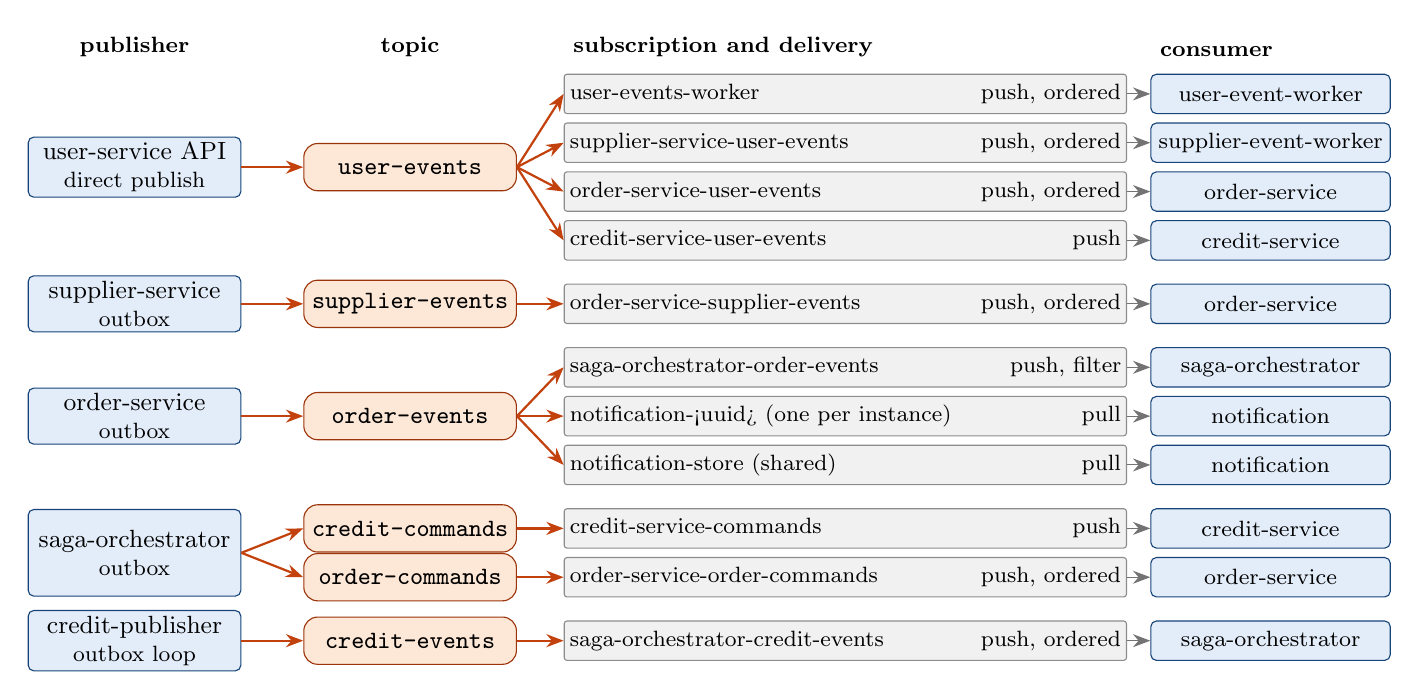
\begin{tikzpicture}[x=1cm,y=1cm]
  % columns: publisher (1.5) | topic (5.0) | subscription (7.15 west) | consumer (15.7)
  \def\rowh{0.62}
  \newcommand{\sub}[4]{%
    \node[subbox, text width=70mm, minimum height=5mm] (s#1) at (6.85,#2) {#3};
    \node[svcbox, font=\footnotesize, text width=29mm, minimum height=5mm, anchor=west] (c#1) at (14.3,#2) {#4};
    \draw[->, draw=black!55] (s#1.east) -- (c#1.west);}
  % user-events
  \sub{1}{0}{\code{user-events-worker}\hfill push, ordered}{user-event-worker}
  \sub{2}{-\rowh}{\code{supplier-service-user-events}\hfill push, ordered}{supplier-event-worker}
  \sub{3}{-2*\rowh}{\code{order-service-user-events}\hfill push, ordered}{order-service}
  \sub{4}{-3*\rowh}{\code{credit-service-user-events}\hfill push}{credit-service}
  \node[topicbox, minimum width=27mm, minimum height=6mm] (t1) at (4.9,-1.5*\rowh) {user-events};
  \node[svcbox, minimum width=27mm, minimum height=6mm] (p1) at (1.4,-1.5*\rowh) {user-service API\\[-1pt]{\footnotesize direct publish}};
  % supplier-events
  \sub{5}{-4.3*\rowh}{\code{order-service-supplier-events}\hfill push, ordered}{order-service}
  \node[topicbox, minimum width=27mm, minimum height=6mm] (t2) at (4.9,-4.3*\rowh) {supplier-events};
  \node[svcbox, minimum width=27mm, minimum height=6mm] (p2) at (1.4,-4.3*\rowh) {supplier-service\\[-1pt]{\footnotesize outbox}};
  % order-events
  \sub{6}{-5.6*\rowh}{\code{saga-orchestrator-order-events}\hfill push, filter}{saga-orchestrator}
  \sub{7}{-6.6*\rowh}{\code{notification-<uuid>} (one per instance)\hfill pull}{notification}
  \sub{8}{-7.6*\rowh}{\code{notification-store} (shared)\hfill pull}{notification}
  \node[topicbox, minimum width=27mm, minimum height=6mm] (t3) at (4.9,-6.6*\rowh) {order-events};
  \node[svcbox, minimum width=27mm, minimum height=6mm] (p3) at (1.4,-6.6*\rowh) {order-service\\[-1pt]{\footnotesize outbox}};
  % credit-commands
  \sub{9}{-8.9*\rowh}{\code{credit-service-commands}\hfill push}{credit-service}
  \node[topicbox, minimum width=27mm, minimum height=6mm] (t4) at (4.9,-8.9*\rowh) {credit-commands};
  % order-commands
  \sub{10}{-9.9*\rowh}{\code{order-service-order-commands}\hfill push, ordered}{order-service}
  \node[topicbox, minimum width=27mm, minimum height=6mm] (t5) at (4.9,-9.9*\rowh) {order-commands};
  \node[svcbox, minimum width=27mm, minimum height=11mm] (p4) at (1.4,-9.4*\rowh) {saga-orchestrator\\[-1pt]{\footnotesize outbox}};
  % credit-events
  \sub{11}{-11.2*\rowh}{\code{saga-orchestrator-credit-events}\hfill push, ordered}{saga-orchestrator}
  \node[topicbox, minimum width=27mm, minimum height=6mm] (t6) at (4.9,-11.2*\rowh) {credit-events};
  \node[svcbox, minimum width=27mm, minimum height=6mm] (p6) at (1.4,-11.2*\rowh) {credit-publisher\\[-1pt]{\footnotesize outbox loop}};
  % arrows
  \draw[asynca] (p1) -- (t1); \draw[asynca] (p2) -- (t2); \draw[asynca] (p3) -- (t3);
  \draw[asynca] (p4.east) -- (t4.west); \draw[asynca] (p4.east) -- (t5.west); \draw[asynca] (p6) -- (t6);
  \foreach \i in {1,2,3,4} \draw[asynca] (t1.east) -- (s\i.west);
  \draw[asynca] (t2) -- (s5);
  \foreach \i in {6,7,8} \draw[asynca] (t3.east) -- (s\i.west);
  \draw[asynca] (t4) -- (s9); \draw[asynca] (t5) -- (s10); \draw[asynca] (t6) -- (s11);
  \node[font=\footnotesize\bfseries, anchor=south] at (1.4,0.35) {publisher};
  \node[font=\footnotesize\bfseries, anchor=south] at (4.9,0.35) {topic};
  \node[font=\footnotesize\bfseries, anchor=south west] at (6.85,0.35) {subscription and delivery};
  \node[font=\footnotesize\bfseries, anchor=south west] at (14.3,0.35) {consumer};
\end{tikzpicture}
\caption{Every topic and subscription. ``Ordered'' means message ordering is enabled. The saga's
filter passes only \code{order.created}, \code{.cancelled}, \code{.expired} and \code{.completed};
both notification subscriptions accept every \code{order.*} type.}
\label{fig:map}
\end{figure}

\section{The seven services and what each sends and receives}

\begin{description}[leftmargin=0pt, labelsep=0.4em, itemsep=2pt, font=\bfseries]
\item[frontend-service (Nuxt).] The only thing the browser loads. Its server routes keep the JWT in
an httpOnly cookie and call the backends; it owns no database and uses no Pub/Sub.
\item[user-service] (API + \code{user-event-worker}). Handles sign-up, login and profiles, and
signs the JWTs. Unusually, the API does not write users to its database: it publishes
\code{user.created}, \code{.updated} or \code{.deleted}, carrying a full user snapshot and a
global \code{version}, and the worker writes the \code{users} table from those events.
\item[supplier-service] (API + \code{supplier-event-worker} + ticker). Admin edits to suppliers
are published to \code{supplier-events} through an outbox. The worker keeps a local copy of users
(for role checks) from \code{user-events} and offers a ``publish leftover outbox rows'' route that
the ticker calls every minute.
\item[order-service] (API + ticker). Owns orders and their state machine. It keeps local copies
of users and of every supplier version, so it can check an order without calling anyone. Every
state change is a row in \code{order_events}, which is both the order history and its outbox, and
is published to \code{order-events}. It obeys saga commands from \code{order-commands}.
\item[saga-orchestrator] (+ ticker). No user API. It reacts to four order event types and to
credit results, keeps one saga row per order, and sends commands through its own outbox. Its
ticker aborts reservations that credit has not answered within 60 seconds.
\item[credit-service] (API + \code{credit-publisher} + one-shot provisioner). Holds balances.
It receives \code{user-events} (to open an account with 1000 credits) and \code{credit-commands}
(reserve, release, transfer), and writes each result to \code{credit_outbox}. A separate
publisher loop sends those rows to \code{credit-events} about once a second.
\item[notification-service.] Pulls \code{order-events}, pushes live updates to browsers over a
WebSocket (\code{/ws}), and stores per-user notifications. Nobody is notified about their own
action.
\end{description}
Each service owns one PostgreSQL database, and no service reads another's. That is why services
learn about each other only through events, and why events carry whole snapshots rather than IDs.

\section{Publishing reliably and acknowledging safely}

\textbf{The outbox.} A service cannot commit a database change and publish to Pub/Sub as one
atomic step. If it tried to do both, a crash in between would lose the message or announce a
change that never happened. So supplier, order, saga and credit write the message as an
\emph{outbox row in the same database transaction} as the business change. A relay then
publishes unpublished rows in order and marks them \code{published_at}. It runs right after
the commit, at startup and on an every-minute sweep (credit's relay is its own process). An
advisory lock allows one relay per database, and a key that fails to publish holds back its
later rows, so per-key order holds. A crash after publishing but before marking the row
publishes the same row again with the same ID. So the guarantee is ``every committed change is
announced \emph{at least} once'', never exactly once.

\textbf{The exception: user-service.} It publishes \emph{instead of} writing its database. If
the publish fails, the request fails and nothing changes. If it succeeds, the user row appears
only after \code{user-event-worker} applies the event, so a login can briefly lag.

\textbf{What counts as an acknowledgement.} Order-service, the saga and the supplier worker
answer \textbf{204} on success and also for a malformed message, which can never succeed and
would otherwise block its ordering key. They answer \textbf{500} when the database fails, so
Pub/Sub retries later. \code{user-event-worker} and credit-service answer \textbf{400} to
malformed input. Pub/Sub retries that too, because no dead-letter topic is configured. Credit
answers \textbf{503} on purpose while waiting for a prerequisite, for example an order's
reservation before its user's account exists. Pub/Sub's redelivery then acts as the wait loop.
Notification-service always acks its live subscription, but acks the store one only after
saving.

\textbf{How duplicates become harmless.} User copies apply an event only if its \code{version}
is newer than the stored one. Supplier versions and notifications insert with ``on conflict do
nothing'' on a natural key. The saga records each \code{eventId} in \code{processed_messages}.
Order-service refuses a second command with the same \code{commandId}. Credit stores every
command under its \code{requestId} and replays the stored result.

\section{End to end: sign-up, supplier edits and the order saga}

\textbf{Sign-up replicates the user to four places.} \code{POST /register} validates the input
and reserves a user ID and event version. It publishes \code{user.created} (key = user ID) and
returns a JWT. Fanout then delivers the event independently, in any order, to four subscriptions.
\code{user-event-worker} writes the login row. The supplier and order workers each upsert a small
copy (id, display name, role) if the version is newer. Credit opens an account with 1000
credits. Until its copy exists, order-service answers \emph{503 ``your account is still being
set up''}, and credit shows its balance as being set up. Deletion soft-deletes the copies, so old
orders can still refer to the user.

\textbf{A supplier edit reaches order-service.} An admin's \code{PUT /suppliers/:id} updates the
row and inserts a \code{supplier.updated} outbox row with the full snapshot in one transaction.
The relay publishes it (key = supplier ID). Order-service \emph{appends} it to
\code{supplier_versions} and never edits old rows. New orders use the latest version, and
existing orders keep the version they were placed against.

\begin{figure}[h]
\centering
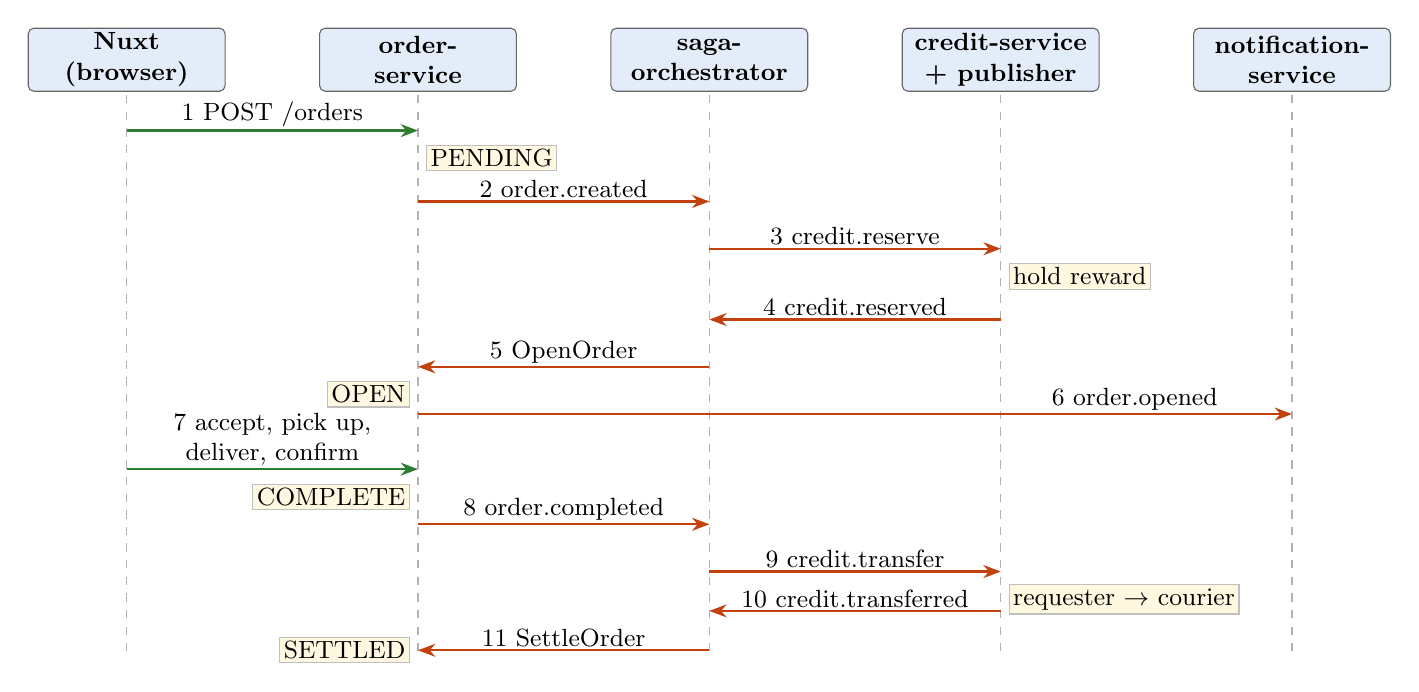
\begin{tikzpicture}[x=1cm,y=0.5cm]
  \foreach \x/\t in {1.2/{Nuxt\\(browser)}, 4.9/{order-\\service}, 8.6/{saga-\\orchestrator}, 12.3/{credit-service\\+ publisher}, 16.0/{notification-\\service}} {
    \node[head] at (\x,0) {\t};
    \draw[life] (\x,-0.9) -- (\x,-15.2);
  }
  \def\N{1.2} \def\O{4.9} \def\S{8.6} \def\C{12.3} \def\T{16.0}
  \draw[mh] (\N,-1.8) -- node[mlab]{1 \code{POST /orders}} (\O,-1.8);
  \node[act, anchor=west] at (\O+0.1,-2.5) {PENDING};
  \draw[m] (\O,-3.6) -- node[mlab]{2 order.created} (\S,-3.6);
  \draw[m] (\S,-4.8) -- node[mlab]{3 credit.reserve} (\C,-4.8);
  \node[act, anchor=west] at (\C+0.1,-5.5) {hold reward};
  \draw[m] (\C,-6.6) -- node[mlab]{4 credit.reserved} (\S,-6.6);
  \draw[m] (\S,-7.8) -- node[mlab]{5 OpenOrder} (\O,-7.8);
  \node[act, anchor=east] at (\O-0.1,-8.5) {OPEN};
  \draw[m] (\O,-9.0) -- node[mlab, pos=0.82]{6 order.opened} (\T,-9.0);
  \draw[mh] (\N,-10.4) -- node[mlab, align=center]{7 accept, pick up,\\deliver, confirm} (\O,-10.4);
  \node[act, anchor=east] at (\O-0.1,-11.1) {COMPLETE};
  \draw[m] (\O,-11.8) -- node[mlab]{8 order.completed} (\S,-11.8);
  \draw[m] (\S,-13.0) -- node[mlab]{9 credit.transfer} (\C,-13.0);
  \node[act, anchor=west] at (\C+0.1,-13.7) {requester $\rightarrow$ courier};
  \draw[m] (\C,-14.0) -- node[mlab, pos=0.5]{10 credit.transferred} (\S,-14.0);
  \draw[m] (\S,-15.0) -- node[mlab]{11 SettleOrder} (\O,-15.0);
  \node[act, anchor=east] at (\O-0.1,-15.0) {SETTLED};
\end{tikzpicture}
\caption{The order saga. Green arrows are HTTP calls; orange arrows are Pub/Sub messages through
the topics in Figure~\ref{fig:map}. Notification-service sees every \code{order.*} event, not
only the one drawn.}
\label{fig:saga}
\end{figure}

\textbf{The order saga} (Figure~\ref{fig:saga}). A \emph{saga} is a business process spread over
several services. Each step is a local transaction, and a later failure is undone by a
\emph{compensating} step rather than a global rollback. (1) The requester's order is stored as
\code{PENDING}, and \code{order.created} goes into the outbox. (2) The saga creates its row in
\code{RESERVING}, with a 60-second deadline, and (3) sends \code{credit.reserve}. Credit checks
that the available credits cover the reward and holds them. (4) Its publisher emits
\code{credit.reserved}. The saga matches the \code{requestId}, moves to \code{OPEN} and (5) sends
\code{OpenOrder}. Order-service opens the order for two hours, and (6) \code{order.opened} reaches
notification-service, which notifies the requester. (7) A courier accepts, picks up and delivers,
and the requester confirms, all over HTTP. The saga's filter skips the intermediate events.
(8)~On \code{order.completed} the saga (9) sends \code{credit.transfer}. Credit moves the held
credits to the courier, (10) reports success, and (11) \code{SettleOrder} marks the order
\code{SETTLED}, which notifies the courier.

\textbf{When it goes wrong.} If credits are short, credit answers
\code{credit.reservation_rejected}, the saga sends \code{RejectOrder}, and nothing needs undoing.
If credit is down, the command waits in its subscription. After 60 seconds the saga ticker
compensates: it sends \code{credit.release} \emph{and} \code{AbortOrder}. When credit returns,
either queued command may run first, because that subscription is unordered. Either way the
credits end up released, thanks to credit's per-order lock and reservation state. A cancelled or
expired order makes the saga send \code{credit.release}. If credit refuses a release or a
transfer, the saga stops in \code{FAILED} with only a log line; nothing retries it.

\section{How each service is containerized}

\textbf{The common pattern.} Every service folder is its own Docker build context, so no image
can contain another service's code. Supplier, order, saga and notification share a three-stage
Dockerfile on \code{node:22-bookworm-slim}. \emph{tooling} installs all dependencies and holds
the TypeScript sources and migrations. \emph{build} compiles to \code{dist/} and drops dev
dependencies. \emph{runtime} copies only \code{dist/} and production modules, runs as the
unprivileged \code{node} user, and starts \code{node dist/index.js}. \code{package*.json} is copied
before the sources, so the slow \code{npm ci} layer is cached when only code changes. Compose
reuses images in two ways: \code{target: tooling} builds the one-shot \code{*-db-migrate}
containers, and \code{command:} replaces the image's default command to start a worker or
publisher from the same image. Table~\ref{tab:containers} lists what differs per service.

\begin{table}[h]
\centering\small
\setlength{\tabcolsep}{4pt}
\begin{tabular}{@{}p{19mm}p{62mm}p{21mm}p{63mm}@{}}
\toprule
Service & Image & Port $\rightarrow$ host & Extra containers from the same image\\
\midrule
frontend & build $\rightarrow$ runtime; ships only Nuxt's \code{.output}; user \code{node}; backend URLs read at start from \code{NUXT_*} env & 3000 $\rightarrow$ 3001 & none\\
user & one stage; all deps; runs TypeScript with \code{tsx}; root & 3333 $\rightarrow$ 3333 & worker (\code{npm run worker}, 3334, unpublished); migrate (\code{drizzle-kit push})\\
supplier & common three-stage & 3000 $\rightarrow$ 3000 & worker (\code{node dist/worker.js}, 3004, unpublished); migrate; \code{tools}-profile seeder\\
order & common three-stage & 3000 $\rightarrow$ 3002 & migrate\\
saga & common three-stage & 3000, none & migrate\\
credit & two stages on \code{node:22-alpine}; reinstalls prod deps; root & 3000 $\rightarrow$ 3004 & publisher; one-shot \code{pubsub:provision}; migrate (from runtime image)\\
notification & common three-stage & 3000 $\rightarrow$ 3003 & migrate\\
\bottomrule
\end{tabular}
\caption{Per-service differences. Supplier, order and saga each also get a tiny
\code{curlimages/curl} ticker: a shell loop of \code{sleep 60; curl -X POST} to an internal sweep route.}
\label{tab:containers}
\end{table}

\textbf{Networking.} \code{compose.yaml} declares no networks, so every container joins one
default network where each \emph{service name} is a DNS name. Containers therefore reach each
other at addresses like \code{http://order-service:3000}, \code{order-db:5432} and
\code{pubsub-emulator:8085}, always on the \emph{container} port. Publishing (\code{"3002:3000"})
is a separate door from the host, and \code{EXPOSE} only documents a port and opens nothing. For
example, the supplier worker listens on 3004 although its image says \code{EXPOSE 3000}, and
\emph{host} port 3004 is credit-service. The browser uses only host ports 3001 (frontend) and 3003
(the notification WebSocket). The emulator and the saga are not published at all. Locally the
emulator cannot sign push requests, so push URLs carry a local-only shared secret instead of
Google's OIDC token.

\textbf{Startup order encodes the subscription rule.} The emulator starts empty and keeps
everything in memory. When \code{PUBSUB_EMULATOR_HOST} is set, each consumer creates its own
topics and subscriptions at startup, and only then starts listening. The provisioner does this
for credit. So a passing \code{/health} check also means ``my subscriptions exist''. Compose uses
\code{depends_on} with \code{service_healthy}, which waits for that check, and with
\code{service_completed_successfully}, which waits for a migration or provisioning job to exit
cleanly. As a result, user-service waits for its worker and for the supplier and order
consumers, supplier-service waits for order-service, and the saga waits for order-service and
the credit provisioner. In each case the readers exist before the first message is published.
One gap: user-service does not wait for the credit provisioner. Restarting only the emulator
loses every subscription until the consumers restart.

\textbf{Persistence.} Six \code{postgres:17} containers, one per service, keep
\code{/var/lib/postgresql/data} in named volumes (\code{order-db-data}, \ldots). They survive
\code{docker compose down}, are deleted by \code{down -v}, and are published only on
\code{127.0.0.1} (5433--5439). The emulator has no volume, so undelivered messages die with it.
\code{compose.dev.yaml} adds hot reloading by syncing \code{src/} into \code{tooling}-stage
containers running \code{tsx watch}. The opt-in \code{compose.tap.yaml} adds the event bus tap
on the same network, where it can reach the unpublished emulator. In Google Cloud the same images
run on Cloud Run with real Pub/Sub, set up by \code{deploy.sh}; that transport is configured but
has no recorded run.

\end{document}
